% Options for packages loaded elsewhere
\PassOptionsToPackage{unicode}{hyperref}
\PassOptionsToPackage{hyphens}{url}
%
\documentclass[
]{article}
\usepackage{amsmath,amssymb}
\usepackage{lmodern}
\usepackage{ifxetex,ifluatex}
\ifnum 0\ifxetex 1\fi\ifluatex 1\fi=0 % if pdftex
  \usepackage[T1]{fontenc}
  \usepackage[utf8]{inputenc}
  \usepackage{textcomp} % provide euro and other symbols
\else % if luatex or xetex
  \usepackage{unicode-math}
  \defaultfontfeatures{Scale=MatchLowercase}
  \defaultfontfeatures[\rmfamily]{Ligatures=TeX,Scale=1}
\fi
% Use upquote if available, for straight quotes in verbatim environments
\IfFileExists{upquote.sty}{\usepackage{upquote}}{}
\IfFileExists{microtype.sty}{% use microtype if available
  \usepackage[]{microtype}
  \UseMicrotypeSet[protrusion]{basicmath} % disable protrusion for tt fonts
}{}
\makeatletter
\@ifundefined{KOMAClassName}{% if non-KOMA class
  \IfFileExists{parskip.sty}{%
    \usepackage{parskip}
  }{% else
    \setlength{\parindent}{0pt}
    \setlength{\parskip}{6pt plus 2pt minus 1pt}}
}{% if KOMA class
  \KOMAoptions{parskip=half}}
\makeatother
\usepackage{xcolor}
\IfFileExists{xurl.sty}{\usepackage{xurl}}{} % add URL line breaks if available
\IfFileExists{bookmark.sty}{\usepackage{bookmark}}{\usepackage{hyperref}}
\hypersetup{
  pdftitle={1992 U.S. Presidential election},
  pdfauthor={Ali Tarek Maher Ibrahim Ali Seada and Paul Lovis Maximilian Trüstedt},
  hidelinks,
  pdfcreator={LaTeX via pandoc}}
\urlstyle{same} % disable monospaced font for URLs
\usepackage[margin=1in]{geometry}
\usepackage{color}
\usepackage{fancyvrb}
\newcommand{\VerbBar}{|}
\newcommand{\VERB}{\Verb[commandchars=\\\{\}]}
\DefineVerbatimEnvironment{Highlighting}{Verbatim}{commandchars=\\\{\}}
% Add ',fontsize=\small' for more characters per line
\usepackage{framed}
\definecolor{shadecolor}{RGB}{248,248,248}
\newenvironment{Shaded}{\begin{snugshade}}{\end{snugshade}}
\newcommand{\AlertTok}[1]{\textcolor[rgb]{0.94,0.16,0.16}{#1}}
\newcommand{\AnnotationTok}[1]{\textcolor[rgb]{0.56,0.35,0.01}{\textbf{\textit{#1}}}}
\newcommand{\AttributeTok}[1]{\textcolor[rgb]{0.77,0.63,0.00}{#1}}
\newcommand{\BaseNTok}[1]{\textcolor[rgb]{0.00,0.00,0.81}{#1}}
\newcommand{\BuiltInTok}[1]{#1}
\newcommand{\CharTok}[1]{\textcolor[rgb]{0.31,0.60,0.02}{#1}}
\newcommand{\CommentTok}[1]{\textcolor[rgb]{0.56,0.35,0.01}{\textit{#1}}}
\newcommand{\CommentVarTok}[1]{\textcolor[rgb]{0.56,0.35,0.01}{\textbf{\textit{#1}}}}
\newcommand{\ConstantTok}[1]{\textcolor[rgb]{0.00,0.00,0.00}{#1}}
\newcommand{\ControlFlowTok}[1]{\textcolor[rgb]{0.13,0.29,0.53}{\textbf{#1}}}
\newcommand{\DataTypeTok}[1]{\textcolor[rgb]{0.13,0.29,0.53}{#1}}
\newcommand{\DecValTok}[1]{\textcolor[rgb]{0.00,0.00,0.81}{#1}}
\newcommand{\DocumentationTok}[1]{\textcolor[rgb]{0.56,0.35,0.01}{\textbf{\textit{#1}}}}
\newcommand{\ErrorTok}[1]{\textcolor[rgb]{0.64,0.00,0.00}{\textbf{#1}}}
\newcommand{\ExtensionTok}[1]{#1}
\newcommand{\FloatTok}[1]{\textcolor[rgb]{0.00,0.00,0.81}{#1}}
\newcommand{\FunctionTok}[1]{\textcolor[rgb]{0.00,0.00,0.00}{#1}}
\newcommand{\ImportTok}[1]{#1}
\newcommand{\InformationTok}[1]{\textcolor[rgb]{0.56,0.35,0.01}{\textbf{\textit{#1}}}}
\newcommand{\KeywordTok}[1]{\textcolor[rgb]{0.13,0.29,0.53}{\textbf{#1}}}
\newcommand{\NormalTok}[1]{#1}
\newcommand{\OperatorTok}[1]{\textcolor[rgb]{0.81,0.36,0.00}{\textbf{#1}}}
\newcommand{\OtherTok}[1]{\textcolor[rgb]{0.56,0.35,0.01}{#1}}
\newcommand{\PreprocessorTok}[1]{\textcolor[rgb]{0.56,0.35,0.01}{\textit{#1}}}
\newcommand{\RegionMarkerTok}[1]{#1}
\newcommand{\SpecialCharTok}[1]{\textcolor[rgb]{0.00,0.00,0.00}{#1}}
\newcommand{\SpecialStringTok}[1]{\textcolor[rgb]{0.31,0.60,0.02}{#1}}
\newcommand{\StringTok}[1]{\textcolor[rgb]{0.31,0.60,0.02}{#1}}
\newcommand{\VariableTok}[1]{\textcolor[rgb]{0.00,0.00,0.00}{#1}}
\newcommand{\VerbatimStringTok}[1]{\textcolor[rgb]{0.31,0.60,0.02}{#1}}
\newcommand{\WarningTok}[1]{\textcolor[rgb]{0.56,0.35,0.01}{\textbf{\textit{#1}}}}
\usepackage{graphicx}
\makeatletter
\def\maxwidth{\ifdim\Gin@nat@width>\linewidth\linewidth\else\Gin@nat@width\fi}
\def\maxheight{\ifdim\Gin@nat@height>\textheight\textheight\else\Gin@nat@height\fi}
\makeatother
% Scale images if necessary, so that they will not overflow the page
% margins by default, and it is still possible to overwrite the defaults
% using explicit options in \includegraphics[width, height, ...]{}
\setkeys{Gin}{width=\maxwidth,height=\maxheight,keepaspectratio}
% Set default figure placement to htbp
\makeatletter
\def\fps@figure{htbp}
\makeatother
\setlength{\emergencystretch}{3em} % prevent overfull lines
\providecommand{\tightlist}{%
  \setlength{\itemsep}{0pt}\setlength{\parskip}{0pt}}
\setcounter{secnumdepth}{-\maxdimen} % remove section numbering
\ifluatex
  \usepackage{selnolig}  % disable illegal ligatures
\fi

\title{1992 U.S. Presidential election}
\author{Ali Tarek Maher Ibrahim Ali Seada and Paul Lovis Maximilian
Trüstedt}
\date{24 6 2021}

\begin{document}
\maketitle

\hypertarget{read-the-data-into-r-environment}{%
\subsection{Read the data into R
environment}\label{read-the-data-into-r-environment}}

\begin{Shaded}
\begin{Highlighting}[]
\FunctionTok{library}\NormalTok{(pacman)}
\FunctionTok{p\_load}\NormalTok{(ggplot2,   }\CommentTok{\# reportable graphs }
\NormalTok{       cowplot,   }\CommentTok{\# arranges ggplot graphs nicely}
\NormalTok{       stargazer, }\CommentTok{\# nice tables}
\NormalTok{       glmnet, }\CommentTok{\# for regularization (lasso, ridge, elastic net)}
\NormalTok{       caret,       }\CommentTok{\#  splitting the data and more}
\NormalTok{       rpart,       }\CommentTok{\#  building decision trees }
\NormalTok{       rpart.plot,}
\NormalTok{       pROC)      }\CommentTok{\# ROC AUC}
\FunctionTok{rm}\NormalTok{(}\AttributeTok{list=}\FunctionTok{ls}\NormalTok{())}
\NormalTok{vote}\OtherTok{\textless{}{-}}\FunctionTok{read.csv}\NormalTok{(}\StringTok{"vote92.csv"}\NormalTok{, }\AttributeTok{sep =} \StringTok{","}\NormalTok{, }\AttributeTok{header =}\NormalTok{ T,}\AttributeTok{stringsAsFactors =}\NormalTok{ T)}
\FunctionTok{str}\NormalTok{(vote)}
\end{Highlighting}
\end{Shaded}

\begin{verbatim}
## 'data.frame':    909 obs. of  10 variables:
##  $ X          : int  1 2 3 4 5 6 7 8 9 10 ...
##  $ vote       : Factor w/ 3 levels "Bush","Clinton",..: 1 1 2 1 2 2 3 1 1 3 ...
##  $ dem        : int  0 0 1 0 0 1 1 0 0 0 ...
##  $ rep        : int  1 1 0 1 0 0 0 1 1 1 ...
##  $ female     : int  1 1 1 0 1 1 1 0 1 0 ...
##  $ persfinance: int  1 0 0 0 0 -1 1 0 1 0 ...
##  $ natlecon   : int  0 -1 -1 -1 -1 -1 0 0 -1 0 ...
##  $ clintondis : num  4.0804 4.0804 1.0404 0.0004 0.9604 ...
##  $ bushdis    : num  0.102 0.102 1.742 5.382 11.022 ...
##  $ perotdis   : num  0.26 0.26 0.24 2.22 6.2 ...
\end{verbatim}

\begin{Shaded}
\begin{Highlighting}[]
\FunctionTok{summary}\NormalTok{(vote)}
\end{Highlighting}
\end{Shaded}

\begin{verbatim}
##        X            vote          dem              rep             female      
##  Min.   :  1   Bush   :310   Min.   :0.0000   Min.   :0.0000   Min.   :0.0000  
##  1st Qu.:228   Clinton:416   1st Qu.:0.0000   1st Qu.:0.0000   1st Qu.:0.0000  
##  Median :455   Perot  :183   Median :0.0000   Median :0.0000   Median :0.0000  
##  Mean   :455                 Mean   :0.4884   Mean   :0.4301   Mean   :0.4752  
##  3rd Qu.:682                 3rd Qu.:1.0000   3rd Qu.:1.0000   3rd Qu.:1.0000  
##  Max.   :909                 Max.   :1.0000   Max.   :1.0000   Max.   :1.0000  
##   persfinance           natlecon         clintondis         bushdis       
##  Min.   :-1.000000   Min.   :-1.0000   Min.   : 0.0004   Min.   : 0.1024  
##  1st Qu.:-1.000000   1st Qu.:-1.0000   1st Qu.: 0.9604   1st Qu.: 0.4624  
##  Median : 0.000000   Median :-1.0000   Median : 1.0404   Median : 1.7424  
##  Mean   :-0.009901   Mean   :-0.6722   Mean   : 3.5062   Mean   : 3.3793  
##  3rd Qu.: 1.000000   3rd Qu.: 0.0000   3rd Qu.: 4.0804   3rd Qu.: 5.3824  
##  Max.   : 1.000000   Max.   : 1.0000   Max.   :16.1600   Max.   :18.6620  
##     perotdis      
##  Min.   : 0.2401  
##  1st Qu.: 0.2401  
##  Median : 2.2201  
##  Mean   : 2.1710  
##  3rd Qu.: 2.2801  
##  Max.   :12.1800
\end{verbatim}

\begin{Shaded}
\begin{Highlighting}[]
\CommentTok{\# ??remove cowplot, stargazer \& pROC}
\end{Highlighting}
\end{Shaded}

\hypertarget{preprocess-the-data-preparing-it-for-the-modeling}{%
\subsection{Preprocess the data, preparing it for the
modeling}\label{preprocess-the-data-preparing-it-for-the-modeling}}

\begin{Shaded}
\begin{Highlighting}[]
\NormalTok{vote}\SpecialCharTok{$}\NormalTok{vote\_num }\OtherTok{\textless{}{-}} \FunctionTok{as.numeric}\NormalTok{(vote}\SpecialCharTok{$}\NormalTok{vote)}
\NormalTok{vote}\SpecialCharTok{$}\NormalTok{dem}\OtherTok{\textless{}{-}}\FunctionTok{as.factor}\NormalTok{(vote}\SpecialCharTok{$}\NormalTok{dem)}
\NormalTok{vote}\SpecialCharTok{$}\NormalTok{rep}\OtherTok{\textless{}{-}}\FunctionTok{as.factor}\NormalTok{(vote}\SpecialCharTok{$}\NormalTok{rep)}
\NormalTok{vote}\SpecialCharTok{$}\NormalTok{female}\OtherTok{\textless{}{-}}\FunctionTok{as.factor}\NormalTok{(vote}\SpecialCharTok{$}\NormalTok{female)}
\NormalTok{vote}\SpecialCharTok{$}\NormalTok{persfinance}\OtherTok{\textless{}{-}}\FunctionTok{as.factor}\NormalTok{(vote}\SpecialCharTok{$}\NormalTok{persfinance)}
\NormalTok{vote}\SpecialCharTok{$}\NormalTok{natlecon}\OtherTok{\textless{}{-}}\FunctionTok{as.factor}\NormalTok{(vote}\SpecialCharTok{$}\NormalTok{natlecon)}
\NormalTok{vote}\SpecialCharTok{$}\NormalTok{polID}\OtherTok{\textless{}{-}}\FunctionTok{as.factor}\NormalTok{((}\FunctionTok{as.numeric}\NormalTok{(vote}\SpecialCharTok{$}\NormalTok{dem)}\SpecialCharTok{{-}}\DecValTok{1}\NormalTok{)}\SpecialCharTok{+}\NormalTok{(}\FunctionTok{as.numeric}\NormalTok{(vote}\SpecialCharTok{$}\NormalTok{rep)}\SpecialCharTok{*}\DecValTok{2{-}1}\NormalTok{))}
\FunctionTok{str}\NormalTok{(vote)}
\end{Highlighting}
\end{Shaded}

\begin{verbatim}
## 'data.frame':    909 obs. of  12 variables:
##  $ X          : int  1 2 3 4 5 6 7 8 9 10 ...
##  $ vote       : Factor w/ 3 levels "Bush","Clinton",..: 1 1 2 1 2 2 3 1 1 3 ...
##  $ dem        : Factor w/ 2 levels "0","1": 1 1 2 1 1 2 2 1 1 1 ...
##  $ rep        : Factor w/ 2 levels "0","1": 2 2 1 2 1 1 1 2 2 2 ...
##  $ female     : Factor w/ 2 levels "0","1": 2 2 2 1 2 2 2 1 2 1 ...
##  $ persfinance: Factor w/ 3 levels "-1","0","1": 3 2 2 2 2 1 3 2 3 2 ...
##  $ natlecon   : Factor w/ 3 levels "-1","0","1": 2 1 1 1 1 1 2 2 1 2 ...
##  $ clintondis : num  4.0804 4.0804 1.0404 0.0004 0.9604 ...
##  $ bushdis    : num  0.102 0.102 1.742 5.382 11.022 ...
##  $ perotdis   : num  0.26 0.26 0.24 2.22 6.2 ...
##  $ vote_num   : num  1 1 2 1 2 2 3 1 1 3 ...
##  $ polID      : Factor w/ 3 levels "1","2","3": 3 3 2 3 1 2 2 3 3 3 ...
\end{verbatim}

We decided to change some of the numeric variables to factors, because
it makes more sense to have them as categorical than as numeric
variables. Also this way, we can see, that there are no problems with
the categorical variables regarding wrong values, because all provided
levels are described by the given data set definition. Additionally we
create a categorical variable called polID to summarize which political
party the respondent is identifying himself with.

\begin{itemize}
\tightlist
\item
  treat missing values
\end{itemize}

\begin{Shaded}
\begin{Highlighting}[]
\FunctionTok{colSums}\NormalTok{(}\FunctionTok{is.na}\NormalTok{(vote))}
\end{Highlighting}
\end{Shaded}

\begin{verbatim}
##           X        vote         dem         rep      female persfinance 
##           0           0           0           0           0           0 
##    natlecon  clintondis     bushdis    perotdis    vote_num       polID 
##           0           0           0           0           0           0
\end{verbatim}

There are no missing values in this data set. No NAs, as well as data,
that could otherwise be identified as missing.

\begin{itemize}
\tightlist
\item
  handle sparse classes of categorical predictors
\end{itemize}

\begin{Shaded}
\begin{Highlighting}[]
\FunctionTok{table}\NormalTok{(vote}\SpecialCharTok{$}\NormalTok{vote) }\CommentTok{\# !!make these tables pretty (bar plot coloured)}
\end{Highlighting}
\end{Shaded}

\begin{verbatim}
## 
##    Bush Clinton   Perot 
##     310     416     183
\end{verbatim}

\begin{Shaded}
\begin{Highlighting}[]
\FunctionTok{table}\NormalTok{(vote}\SpecialCharTok{$}\NormalTok{dem)}
\end{Highlighting}
\end{Shaded}

\begin{verbatim}
## 
##   0   1 
## 465 444
\end{verbatim}

\begin{Shaded}
\begin{Highlighting}[]
\FunctionTok{table}\NormalTok{(vote}\SpecialCharTok{$}\NormalTok{rep)}
\end{Highlighting}
\end{Shaded}

\begin{verbatim}
## 
##   0   1 
## 518 391
\end{verbatim}

\begin{Shaded}
\begin{Highlighting}[]
\FunctionTok{table}\NormalTok{(vote}\SpecialCharTok{$}\NormalTok{female)}
\end{Highlighting}
\end{Shaded}

\begin{verbatim}
## 
##   0   1 
## 477 432
\end{verbatim}

\begin{Shaded}
\begin{Highlighting}[]
\FunctionTok{table}\NormalTok{(vote}\SpecialCharTok{$}\NormalTok{persfinance)}
\end{Highlighting}
\end{Shaded}

\begin{verbatim}
## 
##  -1   0   1 
## 308 302 299
\end{verbatim}

\begin{Shaded}
\begin{Highlighting}[]
\FunctionTok{table}\NormalTok{(vote}\SpecialCharTok{$}\NormalTok{natlecon)}
\end{Highlighting}
\end{Shaded}

\begin{verbatim}
## 
##  -1   0   1 
## 656 208  45
\end{verbatim}

\begin{Shaded}
\begin{Highlighting}[]
\NormalTok{vote}\SpecialCharTok{$}\NormalTok{natlecon[vote}\SpecialCharTok{$}\NormalTok{natlecon}\SpecialCharTok{==}\DecValTok{1}\NormalTok{]}\OtherTok{\textless{}{-}}\DecValTok{0}
\NormalTok{vote}\SpecialCharTok{$}\NormalTok{natlecon[vote}\SpecialCharTok{$}\NormalTok{natlecon}\SpecialCharTok{=={-}}\DecValTok{1}\NormalTok{]}\OtherTok{\textless{}{-}}\DecValTok{1}
\NormalTok{vote}\SpecialCharTok{$}\NormalTok{natlecon}\OtherTok{=}\FunctionTok{droplevels}\NormalTok{(vote}\SpecialCharTok{$}\NormalTok{natlecon)}
\FunctionTok{table}\NormalTok{(vote}\SpecialCharTok{$}\NormalTok{natlecon)}
\end{Highlighting}
\end{Shaded}

\begin{verbatim}
## 
##   0   1 
## 253 656
\end{verbatim}

We leave everything as is except for natlecon which has a sparse class
regarding the level 1. As solution we combine 0 and 1 as the level 0,
meaning national economic conditions have gotten better or stayed the
same over the last 12 months. Level -1 gets changed to 1 as well which
now means that conditions have gotten better. The change from -1 to 1 is
executed just because it is more common to have levels 0 and 1 instead
of 0 and -1.

\begin{itemize}
\tightlist
\item
  take care of outliers, treat the skewed distributions and create new
  features
\end{itemize}

\begin{Shaded}
\begin{Highlighting}[]
\NormalTok{zScores}\OtherTok{\textless{}{-}}\ControlFlowTok{function}\NormalTok{(var) \{}
\NormalTok{    mu}\OtherTok{\textless{}{-}}\FunctionTok{mean}\NormalTok{(var)}
\NormalTok{    sd}\OtherTok{\textless{}{-}}\FunctionTok{sd}\NormalTok{(var)}
    \FunctionTok{return}\NormalTok{((var}\SpecialCharTok{{-}}\NormalTok{mu)}\SpecialCharTok{/}\NormalTok{sd)}
\NormalTok{\}}

\CommentTok{\# treating clintondis}
\NormalTok{tp1}\OtherTok{\textless{}{-}}\FunctionTok{ggplot}\NormalTok{(vote,}\FunctionTok{aes}\NormalTok{(clintondis))}\SpecialCharTok{+}\FunctionTok{geom\_boxplot}\NormalTok{()}\SpecialCharTok{+}\FunctionTok{coord\_flip}\NormalTok{()}
\NormalTok{vote}\SpecialCharTok{$}\NormalTok{clintondis\_fo}\OtherTok{\textless{}{-}}\NormalTok{vote}\SpecialCharTok{$}\NormalTok{clintondis}
\NormalTok{vote}\SpecialCharTok{$}\NormalTok{clintondis\_fo[}\FunctionTok{zScores}\NormalTok{(vote}\SpecialCharTok{$}\NormalTok{clintondis\_fo)}\SpecialCharTok{\textgreater{}}\DecValTok{1}\NormalTok{]}\OtherTok{\textless{}{-}}
    \FunctionTok{round}\NormalTok{(}\FunctionTok{mean}\NormalTok{(vote}\SpecialCharTok{$}\NormalTok{clintondis\_fo))}\SpecialCharTok{+}\FunctionTok{sd}\NormalTok{(vote}\SpecialCharTok{$}\NormalTok{clintondis\_fo)}
\NormalTok{tp2}\OtherTok{\textless{}{-}}\FunctionTok{ggplot}\NormalTok{(vote,}\FunctionTok{aes}\NormalTok{(clintondis\_fo))}\SpecialCharTok{+}\FunctionTok{geom\_boxplot}\NormalTok{()}\SpecialCharTok{+}\FunctionTok{coord\_flip}\NormalTok{()}
\FunctionTok{plot\_grid}\NormalTok{(tp1,tp2,}\AttributeTok{ncol=}\DecValTok{2}\NormalTok{)}
\end{Highlighting}
\end{Shaded}

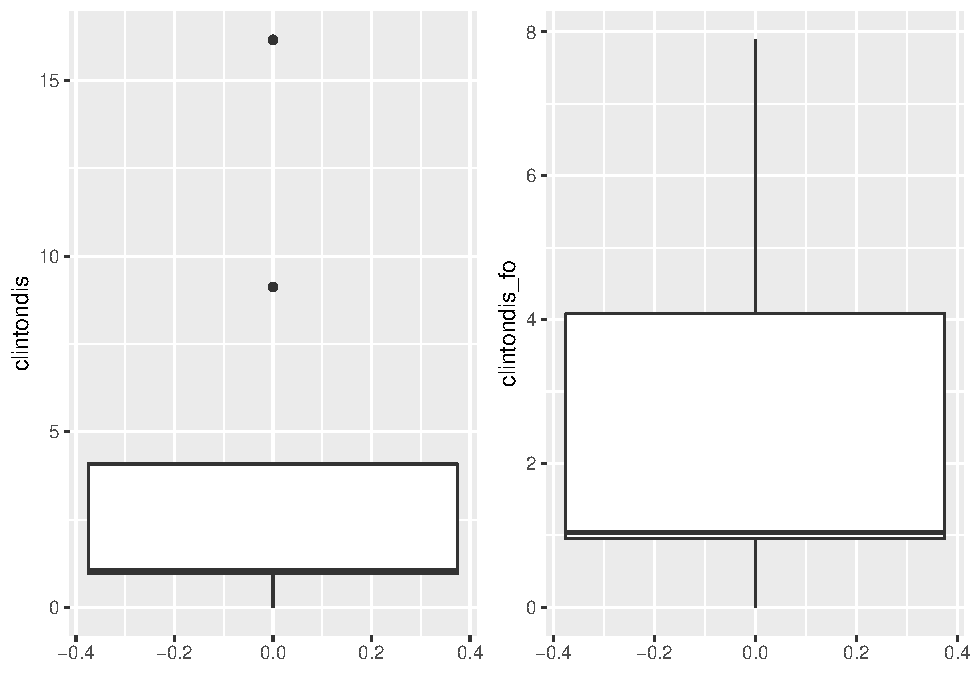
\includegraphics{1992-US-election_files/figure-latex/unnamed-chunk-5-1.pdf}

\begin{Shaded}
\begin{Highlighting}[]
\CommentTok{\# treating bushdis}
\NormalTok{tp1}\OtherTok{\textless{}{-}}\FunctionTok{ggplot}\NormalTok{(vote,}\FunctionTok{aes}\NormalTok{(bushdis))}\SpecialCharTok{+}\FunctionTok{geom\_boxplot}\NormalTok{()}\SpecialCharTok{+}\FunctionTok{coord\_flip}\NormalTok{()}
\NormalTok{vote}\SpecialCharTok{$}\NormalTok{bushdis\_fo}\OtherTok{\textless{}{-}}\NormalTok{vote}\SpecialCharTok{$}\NormalTok{bushdis}
\NormalTok{vote}\SpecialCharTok{$}\NormalTok{bushdis\_fo[}\FunctionTok{zScores}\NormalTok{(vote}\SpecialCharTok{$}\NormalTok{bushdis\_fo)}\SpecialCharTok{\textgreater{}}\DecValTok{2}\NormalTok{]}\OtherTok{\textless{}{-}}
    \FunctionTok{round}\NormalTok{(}\FunctionTok{mean}\NormalTok{(vote}\SpecialCharTok{$}\NormalTok{bushdis\_fo))}\SpecialCharTok{+}\DecValTok{2}\SpecialCharTok{*}\FunctionTok{sd}\NormalTok{(vote}\SpecialCharTok{$}\NormalTok{bushdis\_fo)}
\NormalTok{tp2}\OtherTok{\textless{}{-}}\FunctionTok{ggplot}\NormalTok{(vote,}\FunctionTok{aes}\NormalTok{(bushdis\_fo))}\SpecialCharTok{+}\FunctionTok{geom\_boxplot}\NormalTok{()}\SpecialCharTok{+}\FunctionTok{coord\_flip}\NormalTok{()}
\FunctionTok{plot\_grid}\NormalTok{(tp1,tp2,}\AttributeTok{ncol=}\DecValTok{2}\NormalTok{)}
\end{Highlighting}
\end{Shaded}

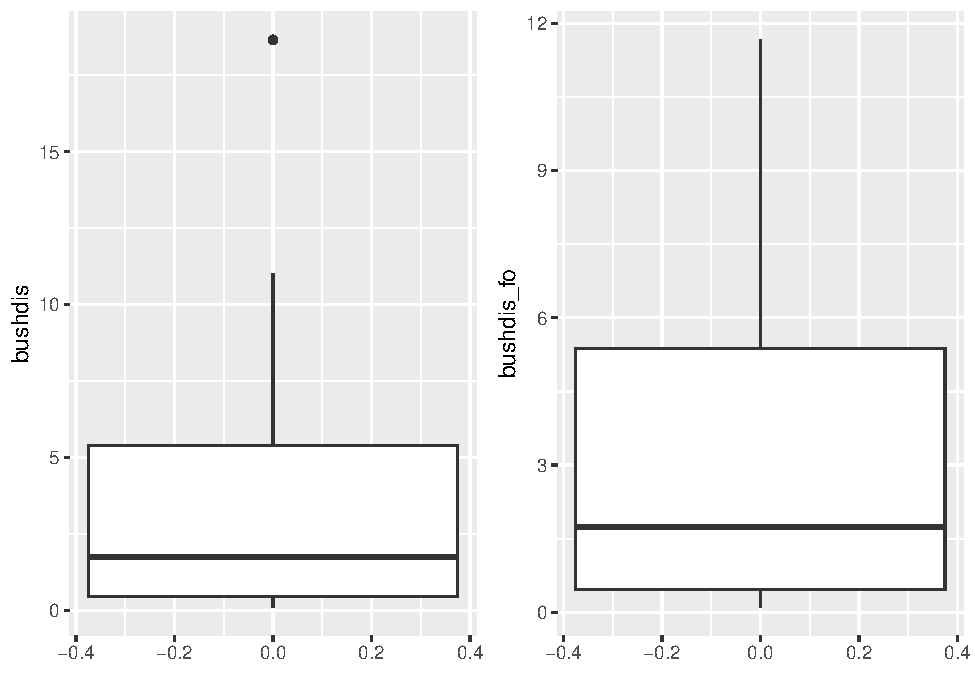
\includegraphics{1992-US-election_files/figure-latex/unnamed-chunk-5-2.pdf}

\begin{Shaded}
\begin{Highlighting}[]
\CommentTok{\# treating perotdis}
\NormalTok{tp1}\OtherTok{\textless{}{-}}\FunctionTok{ggplot}\NormalTok{(vote,}\FunctionTok{aes}\NormalTok{(perotdis))}\SpecialCharTok{+}\FunctionTok{geom\_boxplot}\NormalTok{()}\SpecialCharTok{+}\FunctionTok{coord\_flip}\NormalTok{()}
\NormalTok{vote}\SpecialCharTok{$}\NormalTok{perotdis\_fo}\OtherTok{\textless{}{-}}\NormalTok{vote}\SpecialCharTok{$}\NormalTok{perotdis}
\NormalTok{vote}\SpecialCharTok{$}\NormalTok{perotdis\_fo[}\FunctionTok{zScores}\NormalTok{(vote}\SpecialCharTok{$}\NormalTok{perotdis\_fo)}\SpecialCharTok{\textgreater{}}\DecValTok{1}\NormalTok{]}\OtherTok{\textless{}{-}}
    \FunctionTok{round}\NormalTok{(}\FunctionTok{mean}\NormalTok{(vote}\SpecialCharTok{$}\NormalTok{perotdis\_fo))}\SpecialCharTok{+}\FunctionTok{sd}\NormalTok{(vote}\SpecialCharTok{$}\NormalTok{perotdis\_fo)}
\NormalTok{tp2}\OtherTok{\textless{}{-}}\FunctionTok{ggplot}\NormalTok{(vote,}\FunctionTok{aes}\NormalTok{(perotdis\_fo))}\SpecialCharTok{+}\FunctionTok{geom\_boxplot}\NormalTok{()}\SpecialCharTok{+}\FunctionTok{coord\_flip}\NormalTok{()}
\FunctionTok{plot\_grid}\NormalTok{(tp1,tp2,}\AttributeTok{ncol=}\DecValTok{2}\NormalTok{)}
\end{Highlighting}
\end{Shaded}

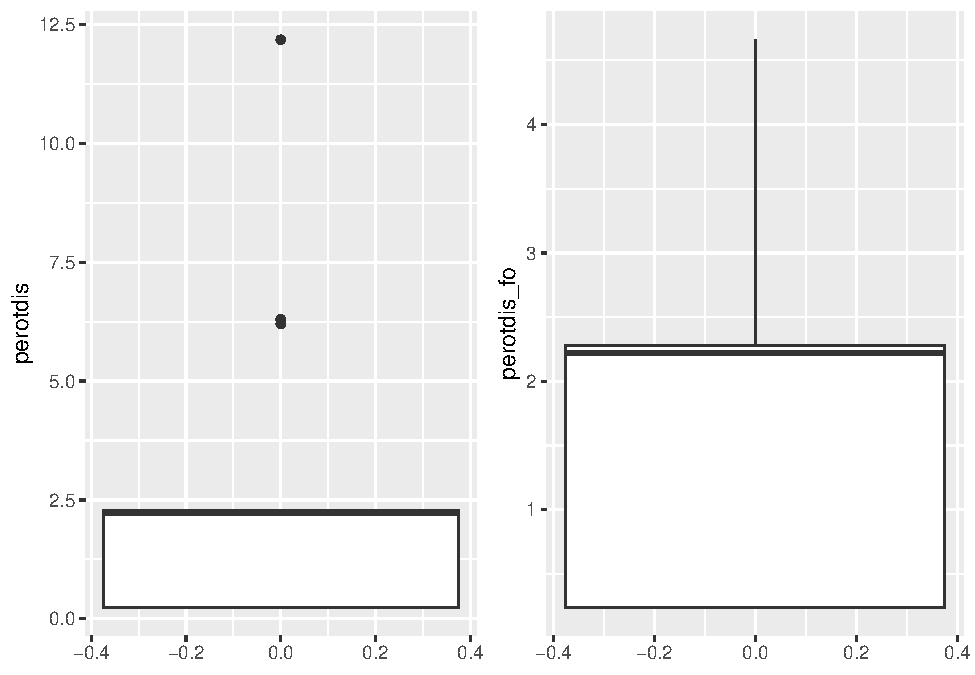
\includegraphics{1992-US-election_files/figure-latex/unnamed-chunk-5-3.pdf}

\begin{Shaded}
\begin{Highlighting}[]
\CommentTok{\# !!make this shit beautiful}
\CommentTok{\# !!reduce the outlier fixes with function}
\end{Highlighting}
\end{Shaded}

There are a few outliers in the variables clintondis, bushdis and
perotdis. We fix those outliers and save the fixed data in the variables
called {[}original\_var\_name{]}\_fo. The ending ``fo'' is derived from
``fixed outliers''.

\begin{itemize}
\tightlist
\item
  explore the relationships between predictors and the target
\end{itemize}

\begin{Shaded}
\begin{Highlighting}[]
\FunctionTok{ggplot}\NormalTok{(vote,}\FunctionTok{aes}\NormalTok{(vote,}\AttributeTok{fill=}\NormalTok{polID))}\SpecialCharTok{+}\FunctionTok{geom\_bar}\NormalTok{() }\CommentTok{\# !!fix colours and descriptions}
\end{Highlighting}
\end{Shaded}

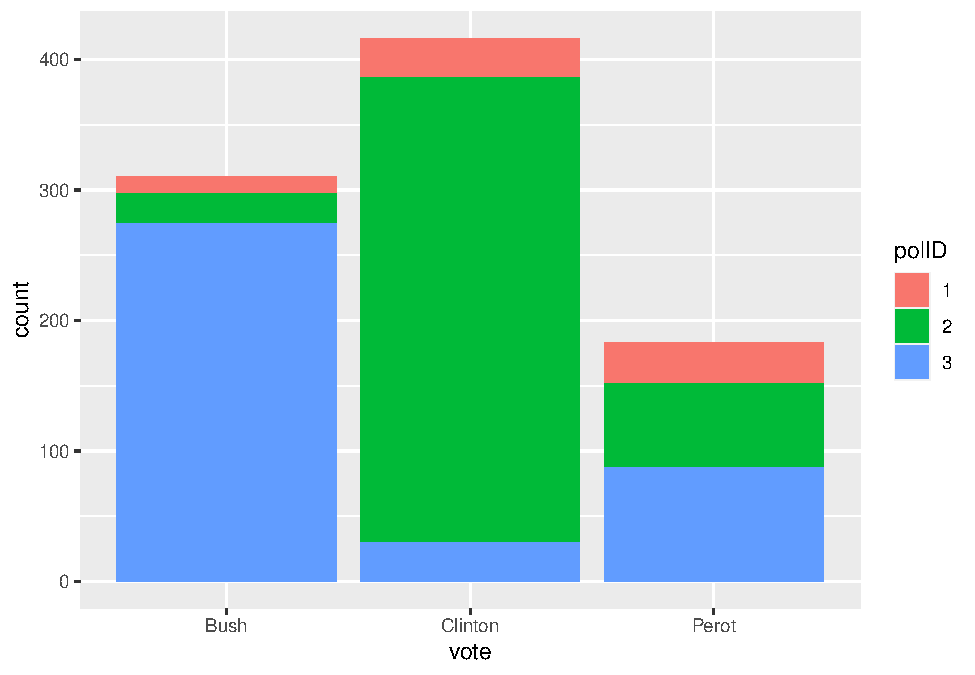
\includegraphics{1992-US-election_files/figure-latex/unnamed-chunk-6-1.pdf}

\begin{Shaded}
\begin{Highlighting}[]
\CommentTok{\# !!add percentiles to those splitted barplots somehow}
\end{Highlighting}
\end{Shaded}

\textbf{\emph{INSERT}}

\begin{Shaded}
\begin{Highlighting}[]
\FunctionTok{ggplot}\NormalTok{(vote,}\FunctionTok{aes}\NormalTok{(vote,}\AttributeTok{fill=}\NormalTok{female))}\SpecialCharTok{+}\FunctionTok{geom\_bar}\NormalTok{()}
\end{Highlighting}
\end{Shaded}

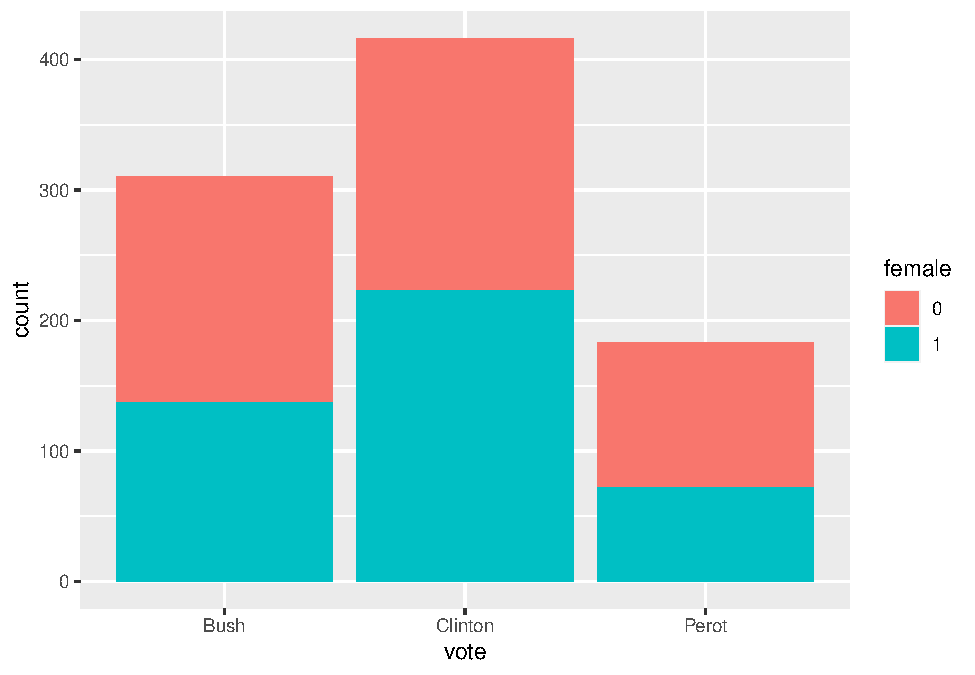
\includegraphics{1992-US-election_files/figure-latex/unnamed-chunk-7-1.pdf}
\textbf{\emph{INSERT}}

\begin{Shaded}
\begin{Highlighting}[]
\NormalTok{p1}\OtherTok{\textless{}{-}}\FunctionTok{ggplot}\NormalTok{(vote,}\FunctionTok{aes}\NormalTok{(vote,}\AttributeTok{fill=}\NormalTok{persfinance))}\SpecialCharTok{+}\FunctionTok{geom\_bar}\NormalTok{()}
\NormalTok{p2}\OtherTok{\textless{}{-}}\FunctionTok{ggplot}\NormalTok{(vote,}\FunctionTok{aes}\NormalTok{(vote,}\AttributeTok{fill=}\NormalTok{natlecon))}\SpecialCharTok{+}\FunctionTok{geom\_bar}\NormalTok{()}
\FunctionTok{plot\_grid}\NormalTok{(p1,p2,}\AttributeTok{ncol=}\DecValTok{2}\NormalTok{)}
\end{Highlighting}
\end{Shaded}

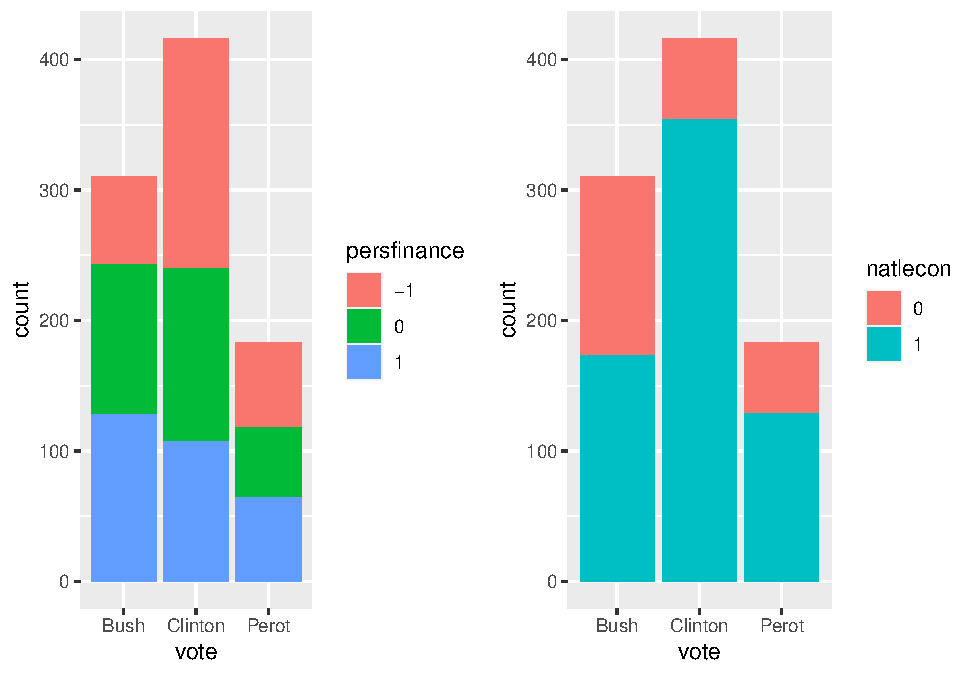
\includegraphics{1992-US-election_files/figure-latex/unnamed-chunk-8-1.pdf}

\begin{Shaded}
\begin{Highlighting}[]
\CommentTok{\# !!fix repeating barplot by creating a more diverse visual representation}
\end{Highlighting}
\end{Shaded}

\textbf{\emph{INSERT}}

\begin{Shaded}
\begin{Highlighting}[]
\NormalTok{p1}\OtherTok{\textless{}{-}}\FunctionTok{ggplot}\NormalTok{(vote,}\FunctionTok{aes}\NormalTok{(clintondis\_fo,}\AttributeTok{fill=}\NormalTok{vote))}\SpecialCharTok{+}\FunctionTok{geom\_histogram}\NormalTok{(}\AttributeTok{bins=}\DecValTok{3}\NormalTok{)}
\NormalTok{p2}\OtherTok{\textless{}{-}}\FunctionTok{ggplot}\NormalTok{(vote,}\FunctionTok{aes}\NormalTok{(bushdis\_fo,}\AttributeTok{fill=}\NormalTok{vote))}\SpecialCharTok{+}\FunctionTok{geom\_histogram}\NormalTok{(}\AttributeTok{bins=}\DecValTok{3}\NormalTok{)}
\NormalTok{p3}\OtherTok{\textless{}{-}}\FunctionTok{ggplot}\NormalTok{(vote,}\FunctionTok{aes}\NormalTok{(perotdis\_fo,}\AttributeTok{fill=}\NormalTok{vote))}\SpecialCharTok{+}\FunctionTok{geom\_histogram}\NormalTok{(}\AttributeTok{bins=}\DecValTok{3}\NormalTok{)}
\NormalTok{p4}\OtherTok{\textless{}{-}}\FunctionTok{ggplot}\NormalTok{(vote,}\FunctionTok{aes}\NormalTok{(clintondis,}\AttributeTok{fill=}\NormalTok{vote))}\SpecialCharTok{+}\FunctionTok{geom\_histogram}\NormalTok{(}\AttributeTok{bins=}\DecValTok{3}\NormalTok{)}
\NormalTok{p5}\OtherTok{\textless{}{-}}\FunctionTok{ggplot}\NormalTok{(vote,}\FunctionTok{aes}\NormalTok{(bushdis,}\AttributeTok{fill=}\NormalTok{vote))}\SpecialCharTok{+}\FunctionTok{geom\_histogram}\NormalTok{(}\AttributeTok{bins=}\DecValTok{3}\NormalTok{)}
\NormalTok{p6}\OtherTok{\textless{}{-}}\FunctionTok{ggplot}\NormalTok{(vote,}\FunctionTok{aes}\NormalTok{(perotdis,}\AttributeTok{fill=}\NormalTok{vote))}\SpecialCharTok{+}\FunctionTok{geom\_histogram}\NormalTok{(}\AttributeTok{bins=}\DecValTok{3}\NormalTok{)}
\FunctionTok{plot\_grid}\NormalTok{(p1,p2,p3,p4,p5,p6,}\AttributeTok{ncol=}\DecValTok{3}\NormalTok{)}
\end{Highlighting}
\end{Shaded}

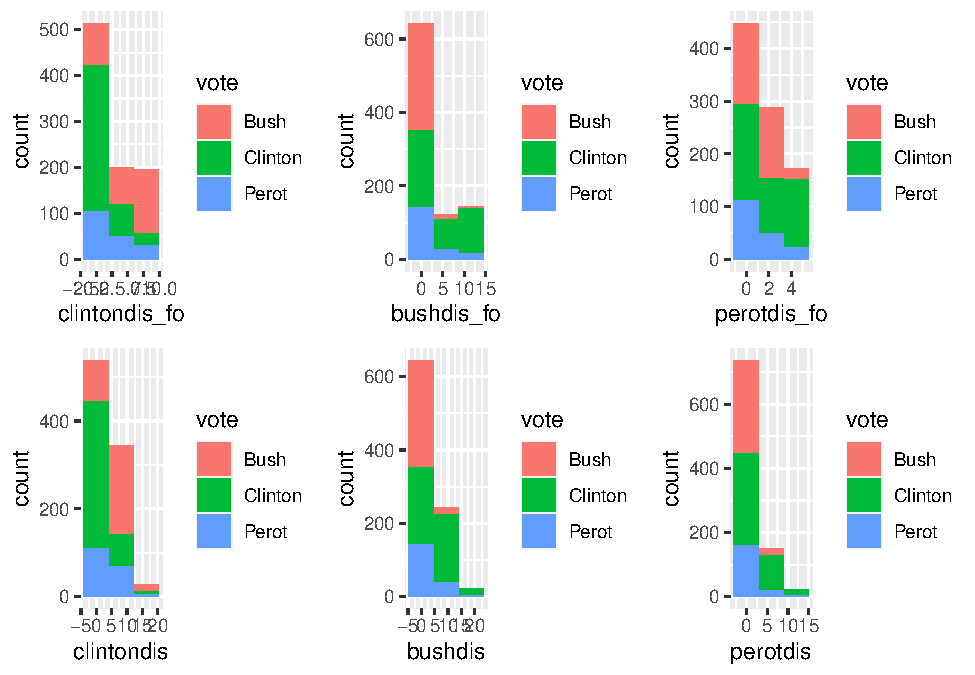
\includegraphics{1992-US-election_files/figure-latex/unnamed-chunk-9-1.pdf}

\begin{Shaded}
\begin{Highlighting}[]
\CommentTok{\# !!fix legend print and axis descriptions, also colours}
\end{Highlighting}
\end{Shaded}

\textbf{\emph{INSERT}}

\hypertarget{building-the-models}{%
\subsection{Building the models}\label{building-the-models}}

\begin{Shaded}
\begin{Highlighting}[]
\CommentTok{\# splitting the data into train and test}
\FunctionTok{set.seed}\NormalTok{(}\DecValTok{777}\NormalTok{)}
\NormalTok{train.Index }\OtherTok{\textless{}{-}}  \FunctionTok{sample}\NormalTok{(}\DecValTok{1}\SpecialCharTok{:}\FunctionTok{nrow}\NormalTok{(vote), }\FunctionTok{round}\NormalTok{(}\FloatTok{0.7}\SpecialCharTok{*}\FunctionTok{nrow}\NormalTok{(vote)), }\AttributeTok{replace =}\NormalTok{ F)}
\CommentTok{\# creating the train and test sets using train.Index }
\NormalTok{vote.train }\OtherTok{\textless{}{-}}\NormalTok{ vote[train.Index,]}
\NormalTok{vote.test  }\OtherTok{\textless{}{-}}\NormalTok{ vote[}\SpecialCharTok{{-}}\NormalTok{train.Index,]}
  
\CommentTok{\# creating x and y for model training}
\CommentTok{\# y {-} a target vector}
\NormalTok{y.train }\OtherTok{\textless{}{-}}\NormalTok{ vote.train}\SpecialCharTok{$}\NormalTok{vote\_num}
\NormalTok{y.test  }\OtherTok{\textless{}{-}}\NormalTok{ vote.test}\SpecialCharTok{$}\NormalTok{vote\_num}

\CommentTok{\# X {-} a matrix with features/predictors }
\NormalTok{features }\OtherTok{\textless{}{-}} \FunctionTok{c}\NormalTok{(}\StringTok{\textquotesingle{}dem\textquotesingle{}}\NormalTok{,}\StringTok{\textquotesingle{}rep\textquotesingle{}}\NormalTok{,}\StringTok{\textquotesingle{}female\textquotesingle{}}\NormalTok{,}\StringTok{\textquotesingle{}persfinance\textquotesingle{}}\NormalTok{,}\StringTok{\textquotesingle{}natlecon\textquotesingle{}}\NormalTok{, }
              \StringTok{\textquotesingle{}clintondis\_fo\textquotesingle{}}\NormalTok{, }\StringTok{\textquotesingle{}bushdis\_fo\textquotesingle{}}\NormalTok{,}\StringTok{\textquotesingle{}perotdis\_fo\textquotesingle{}}\NormalTok{,}\StringTok{\textquotesingle{}polID\textquotesingle{}}\NormalTok{)}


\CommentTok{\#model.matrix( \textasciitilde{} ., data = scoring.train[, features])}
\NormalTok{X.train }\OtherTok{\textless{}{-}} \FunctionTok{model.matrix}\NormalTok{( }\SpecialCharTok{\textasciitilde{}}\NormalTok{ . }\SpecialCharTok{{-}}\DecValTok{1}\NormalTok{, }\AttributeTok{data =}\NormalTok{ vote.train[, features])}
\NormalTok{X.test  }\OtherTok{\textless{}{-}} \FunctionTok{model.matrix}\NormalTok{( }\SpecialCharTok{\textasciitilde{}}\NormalTok{ . }\SpecialCharTok{{-}}\DecValTok{1}\NormalTok{, }\AttributeTok{data =}\NormalTok{ vote.test[, features])}
\end{Highlighting}
\end{Shaded}

\begin{enumerate}
\def\labelenumi{\arabic{enumi}.}
\tightlist
\item
  L1-nrom / Lasso
\end{enumerate}

\begin{Shaded}
\begin{Highlighting}[]
\NormalTok{log\_l1 }\OtherTok{\textless{}{-}} \FunctionTok{glmnet}\NormalTok{(X.train, y.train, }\AttributeTok{alpha =} \DecValTok{1}\NormalTok{)}

\FunctionTok{plot}\NormalTok{(log\_l1, }\AttributeTok{xvar =} \StringTok{"lambda"}\NormalTok{)}
\FunctionTok{legend}\NormalTok{(}\StringTok{"bottomright"}\NormalTok{, }\AttributeTok{lwd =} \DecValTok{1}\NormalTok{, }\AttributeTok{col =} \DecValTok{1}\SpecialCharTok{:}\DecValTok{6}\NormalTok{, }\AttributeTok{legend =} \FunctionTok{colnames}\NormalTok{(X.train), }\AttributeTok{cex =}\NormalTok{ .}\DecValTok{4}\NormalTok{)}
\end{Highlighting}
\end{Shaded}

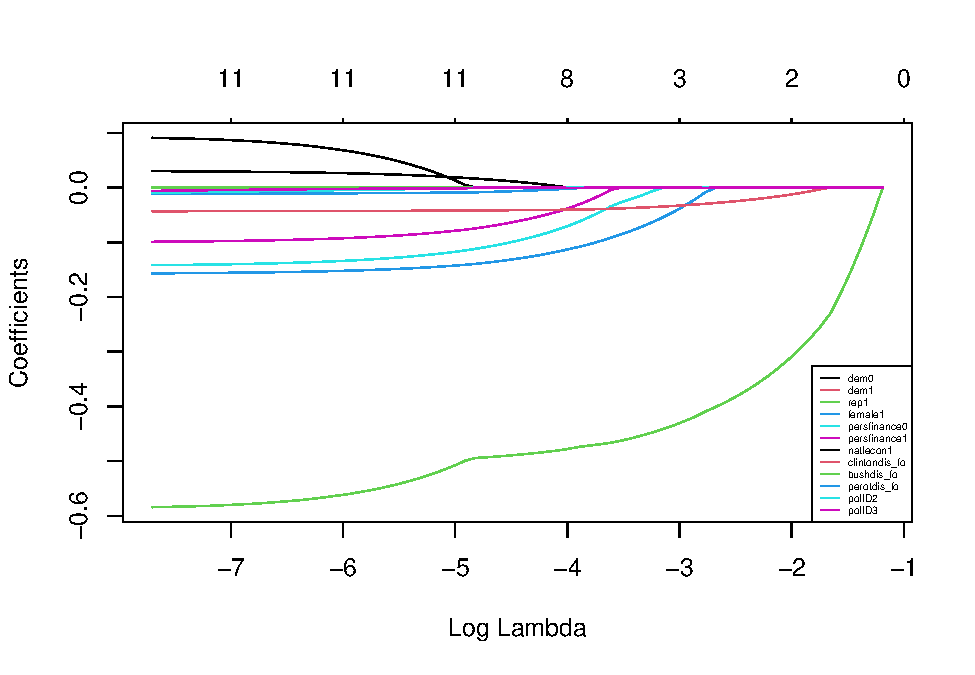
\includegraphics{1992-US-election_files/figure-latex/unnamed-chunk-11-1.pdf}

\begin{Shaded}
\begin{Highlighting}[]
\FunctionTok{plot}\NormalTok{(}\AttributeTok{y =}\NormalTok{ log\_l1}\SpecialCharTok{$}\NormalTok{dev.ratio, }
     \AttributeTok{x =}\NormalTok{ log\_l1}\SpecialCharTok{$}\NormalTok{lambda,}
     \AttributeTok{xlab =} \StringTok{"lambda"}\NormalTok{,}
     \AttributeTok{ylab =} \StringTok{"R{-}squared"}\NormalTok{)}
\end{Highlighting}
\end{Shaded}

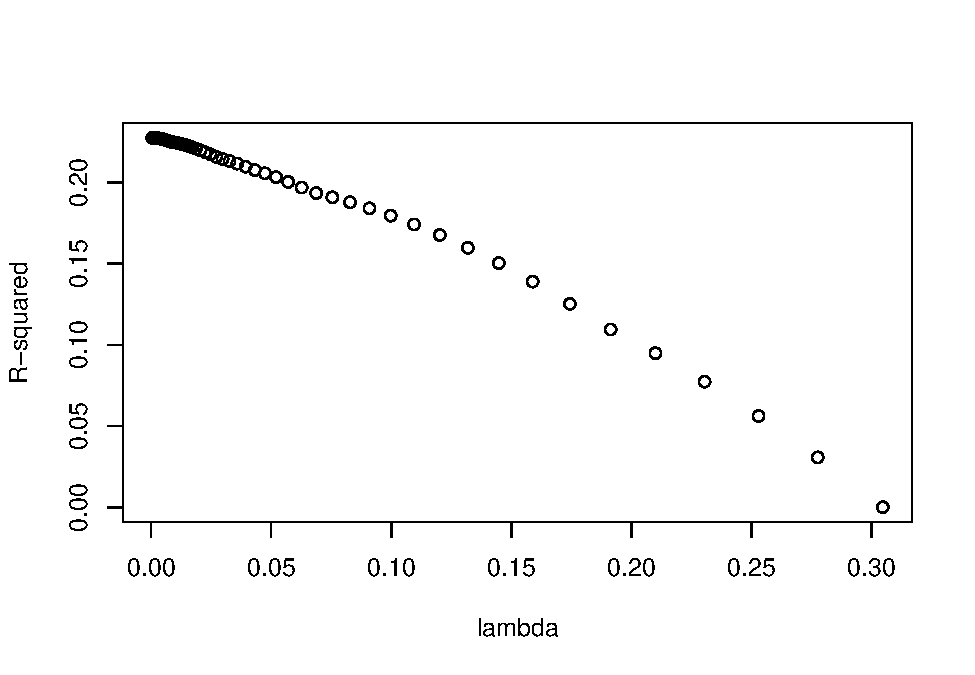
\includegraphics{1992-US-election_files/figure-latex/unnamed-chunk-11-2.pdf}

\begin{Shaded}
\begin{Highlighting}[]
\CommentTok{\# selecting the optimal lambda}
\FunctionTok{set.seed}\NormalTok{(}\DecValTok{77}\NormalTok{)}
\NormalTok{log\_l1\_cv }\OtherTok{\textless{}{-}} \FunctionTok{cv.glmnet}\NormalTok{(X.train, y.train, }\AttributeTok{alpha =} \DecValTok{1}\NormalTok{, }\AttributeTok{type.measure =} \StringTok{"class"}\NormalTok{, }
                       \AttributeTok{lambda =} \DecValTok{10}\SpecialCharTok{\^{}}\FunctionTok{seq}\NormalTok{(}\SpecialCharTok{{-}}\DecValTok{5}\NormalTok{, }\DecValTok{1}\NormalTok{, }\AttributeTok{length.out =} \DecValTok{100}\NormalTok{) , }\AttributeTok{nfolds =} \DecValTok{10}\NormalTok{)}
\end{Highlighting}
\end{Shaded}

\begin{verbatim}
## Warning: Only mse, deviance, mae available as type.measure for Gaussian models;
## mse used instead
\end{verbatim}

\begin{Shaded}
\begin{Highlighting}[]
\NormalTok{y.predlog\_l1 }\OtherTok{\textless{}{-}}  \FunctionTok{predict}\NormalTok{(log\_l1, }\AttributeTok{newx =}\NormalTok{ X.test, }
                         \AttributeTok{type =} \StringTok{"response"}\NormalTok{, }\AttributeTok{s =}\NormalTok{ log\_l1\_cv}\SpecialCharTok{$}\NormalTok{lambda.min)}
\end{Highlighting}
\end{Shaded}

\begin{Shaded}
\begin{Highlighting}[]
\CommentTok{\# Setting alpha = 0 implements ridge regression}
\NormalTok{log\_r1 }\OtherTok{\textless{}{-}} \FunctionTok{glmnet}\NormalTok{(X.train, y.train, }\AttributeTok{alpha =} \DecValTok{0}\NormalTok{)}


\FunctionTok{plot}\NormalTok{(log\_r1, }\AttributeTok{xvar =} \StringTok{"lambda"}\NormalTok{)}
\FunctionTok{legend}\NormalTok{(}\StringTok{"bottomright"}\NormalTok{, }\AttributeTok{lwd =} \DecValTok{1}\NormalTok{, }\AttributeTok{col =} \DecValTok{1}\SpecialCharTok{:}\DecValTok{6}\NormalTok{, }\AttributeTok{legend =} \FunctionTok{colnames}\NormalTok{(X.test), }\AttributeTok{cex =}\NormalTok{ .}\DecValTok{3}\NormalTok{)}
\end{Highlighting}
\end{Shaded}

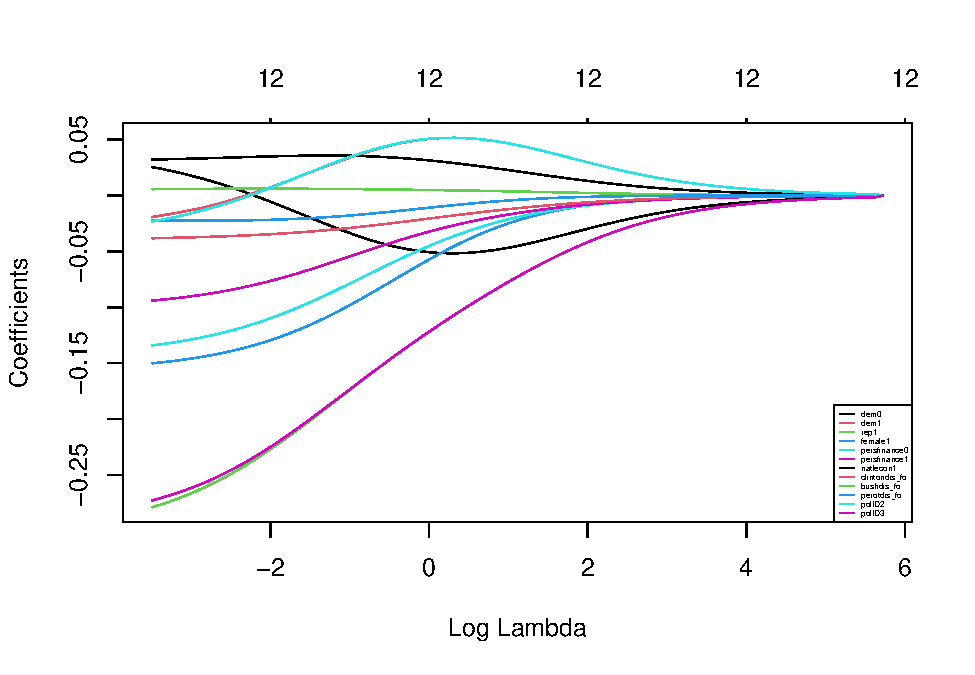
\includegraphics{1992-US-election_files/figure-latex/unnamed-chunk-12-1.pdf}

\begin{Shaded}
\begin{Highlighting}[]
\FunctionTok{plot}\NormalTok{(}\AttributeTok{y =}\NormalTok{ log\_r1}\SpecialCharTok{$}\NormalTok{dev.ratio, }
     \AttributeTok{x =}\NormalTok{ log\_r1}\SpecialCharTok{$}\NormalTok{lambda,}
     \AttributeTok{xlab =} \StringTok{"lambda"}\NormalTok{,}
     \AttributeTok{ylab =} \StringTok{"R{-}squared"}\NormalTok{)}
\end{Highlighting}
\end{Shaded}

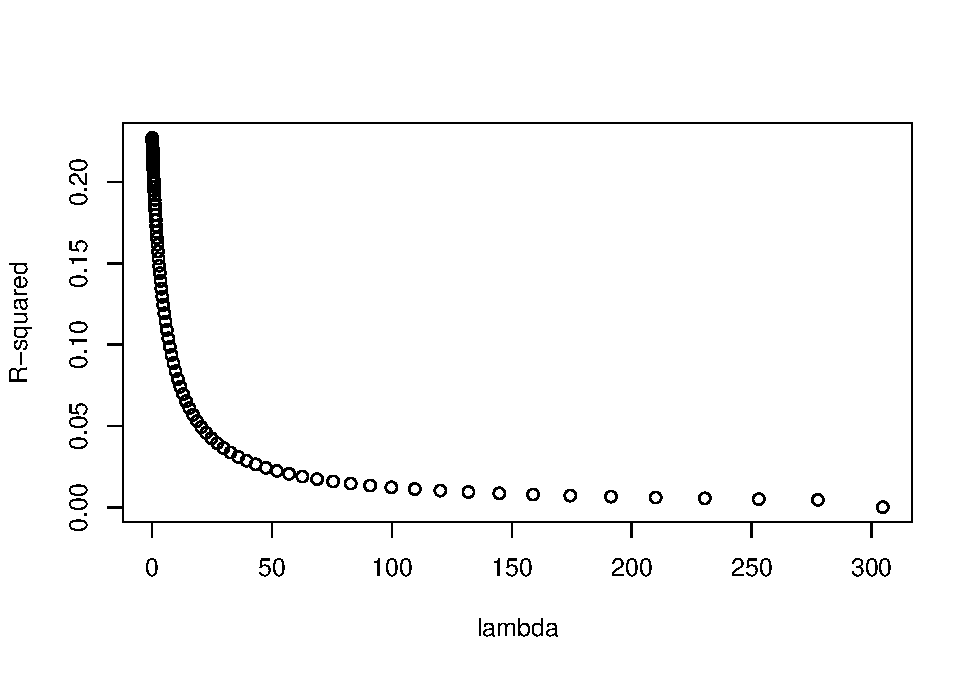
\includegraphics{1992-US-election_files/figure-latex/unnamed-chunk-12-2.pdf}

\begin{Shaded}
\begin{Highlighting}[]
\CommentTok{\# selecting the optimal lambda}
\FunctionTok{set.seed}\NormalTok{(}\DecValTok{77}\NormalTok{)}
\NormalTok{log\_r1\_cv }\OtherTok{\textless{}{-}} \FunctionTok{cv.glmnet}\NormalTok{(X.train, y.train, }\AttributeTok{alpha =} \DecValTok{0}\NormalTok{, }\AttributeTok{type.measure =} \StringTok{"class"}\NormalTok{, }
                       \AttributeTok{lambda =} \DecValTok{10}\SpecialCharTok{\^{}}\FunctionTok{seq}\NormalTok{(}\SpecialCharTok{{-}}\DecValTok{5}\NormalTok{, }\DecValTok{1}\NormalTok{, }\AttributeTok{length.out =} \DecValTok{100}\NormalTok{), }
                        \AttributeTok{nfolds =} \DecValTok{10}\NormalTok{)}
\end{Highlighting}
\end{Shaded}

\begin{verbatim}
## Warning: Only mse, deviance, mae available as type.measure for Gaussian models;
## mse used instead
\end{verbatim}

\begin{Shaded}
\begin{Highlighting}[]
\NormalTok{y.predlog\_r1 }\OtherTok{\textless{}{-}}  \FunctionTok{predict}\NormalTok{(log\_r1,    }\AttributeTok{newx =}\NormalTok{ X.test, }
                         \AttributeTok{type =} \StringTok{"response"}\NormalTok{, }\AttributeTok{s =}\NormalTok{ log\_r1\_cv}\SpecialCharTok{$}\NormalTok{lambda.min)}
\end{Highlighting}
\end{Shaded}

\begin{Shaded}
\begin{Highlighting}[]
\CommentTok{\#only both }

\NormalTok{log1 }\OtherTok{\textless{}{-}} \FunctionTok{glm}\NormalTok{(vote\_num }\SpecialCharTok{\textasciitilde{}}\NormalTok{  dem }\SpecialCharTok{+}\NormalTok{ rep }\SpecialCharTok{+}\NormalTok{ female }\SpecialCharTok{+}\NormalTok{ persfinance }\SpecialCharTok{+} 
\NormalTok{              natlecon }\SpecialCharTok{+}\NormalTok{ clintondis\_fo }\SpecialCharTok{+}\NormalTok{ persfinance }\SpecialCharTok{+}\NormalTok{ perotdis\_fo }\SpecialCharTok{+}\NormalTok{bushdis\_fo,}
           \AttributeTok{data =}\NormalTok{ vote)}
\CommentTok{\#catagorical}
\NormalTok{log2 }\OtherTok{\textless{}{-}} \FunctionTok{glm}\NormalTok{(vote\_num }\SpecialCharTok{\textasciitilde{}}\NormalTok{ dem }\SpecialCharTok{+}\NormalTok{ rep }\SpecialCharTok{+}\NormalTok{ female }\SpecialCharTok{+}\NormalTok{persfinance }\SpecialCharTok{+}
\NormalTok{          natlecon ,}
           \AttributeTok{data =}\NormalTok{ vote)}

\CommentTok{\#only continous}
\NormalTok{log3 }\OtherTok{\textless{}{-}} \FunctionTok{glm}\NormalTok{(vote\_num }\SpecialCharTok{\textasciitilde{}}\NormalTok{ clintondis\_fo }\SpecialCharTok{+}\NormalTok{ bushdis\_fo }\SpecialCharTok{+}
\NormalTok{              perotdis\_fo,}
           \AttributeTok{data =}\NormalTok{ vote)}


\NormalTok{pred.log1 }\OtherTok{\textless{}{-}} \FunctionTok{predict}\NormalTok{(log1, vote, }\AttributeTok{type =} \StringTok{"response"}\NormalTok{)}
\NormalTok{pred.log2 }\OtherTok{\textless{}{-}} \FunctionTok{predict}\NormalTok{(log2, vote, }\AttributeTok{type =} \StringTok{"response"}\NormalTok{)}
\NormalTok{pred.log3 }\OtherTok{\textless{}{-}} \FunctionTok{predict}\NormalTok{(log3, vote, }\AttributeTok{type =} \StringTok{"response"}\NormalTok{)}
\end{Highlighting}
\end{Shaded}

\begin{Shaded}
\begin{Highlighting}[]
\FunctionTok{set.seed}\NormalTok{(}\DecValTok{7}\NormalTok{)}
\NormalTok{train.Index }\OtherTok{\textless{}{-}}\NormalTok{ caret}\SpecialCharTok{::}\FunctionTok{createDataPartition}\NormalTok{(vote}\SpecialCharTok{$}\NormalTok{vote, }\AttributeTok{p =} \FloatTok{0.7}\NormalTok{, }\AttributeTok{list =}\NormalTok{ F)}
\NormalTok{vote.train }\OtherTok{\textless{}{-}}\NormalTok{ vote[ train.Index,]}
\NormalTok{vote.test  }\OtherTok{\textless{}{-}}\NormalTok{ vote[}\SpecialCharTok{{-}}\NormalTok{train.Index,]}

\CommentTok{\# features to be used for model training   }
\NormalTok{features }\OtherTok{\textless{}{-}} \FunctionTok{c}\NormalTok{(}\StringTok{\textquotesingle{}vote\textquotesingle{}}\NormalTok{, }\StringTok{\textquotesingle{}dem\textquotesingle{}}\NormalTok{,}\StringTok{\textquotesingle{}rep\textquotesingle{}}\NormalTok{,}\StringTok{\textquotesingle{}female\textquotesingle{}}\NormalTok{,}\StringTok{\textquotesingle{}persfinance\textquotesingle{}}\NormalTok{,}\StringTok{\textquotesingle{}natlecon\textquotesingle{}}\NormalTok{, }
              \StringTok{\textquotesingle{}clintondis\_fo\textquotesingle{}}\NormalTok{, }\StringTok{\textquotesingle{}bushdis\_fo\textquotesingle{}}\NormalTok{,}\StringTok{\textquotesingle{}perotdis\_fo\textquotesingle{}}\NormalTok{,}\StringTok{\textquotesingle{}polID\textquotesingle{}}\NormalTok{) }

\CommentTok{\# {-}{-}{-}{-}{-} Fitting a model {-}{-}{-}{-}{-}{-} }
\CommentTok{\# Training classification decision tree}
\NormalTok{dt }\OtherTok{\textless{}{-}} \FunctionTok{rpart}\NormalTok{(vote }\SpecialCharTok{\textasciitilde{}}\NormalTok{ ., }
            \AttributeTok{data =}\NormalTok{ vote.train[,features], }
            \AttributeTok{method =} \StringTok{"class"}\NormalTok{,   }\CommentTok{\#cause we have a classification problem}
            \AttributeTok{parms =} \FunctionTok{list}\NormalTok{(}\AttributeTok{split =} \StringTok{"information"}\NormalTok{),  }\CommentTok{\# the splitting index }
            \AttributeTok{model =}\NormalTok{ T) }

\CommentTok{\# {-}{-}{-}{-}{-} Deriving Predictions {-}{-}{-}{-}{-}{-} }

\NormalTok{pred.dt }\OtherTok{\textless{}{-}} \FunctionTok{predict}\NormalTok{(dt, }\AttributeTok{newdata =}\NormalTok{ vote.test, }\AttributeTok{type =} \StringTok{"prob"}\NormalTok{)[, }\DecValTok{2}\NormalTok{]}

\CommentTok{\# Visualizing the results from "dt" using the prp() function}
\CommentTok{\# default plot}
\FunctionTok{prp}\NormalTok{(dt)}
\end{Highlighting}
\end{Shaded}

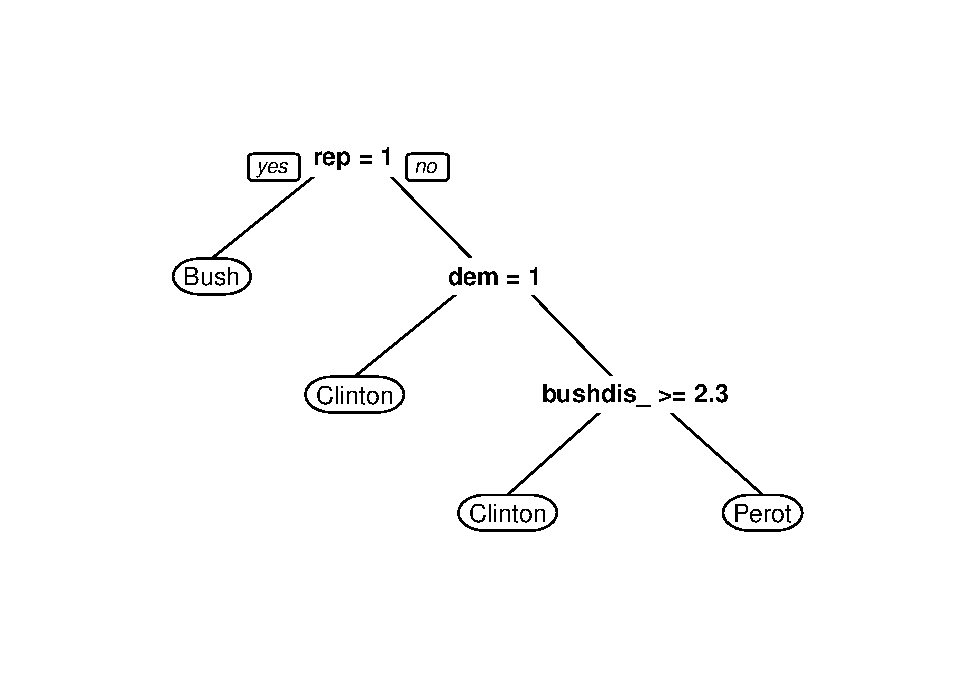
\includegraphics{1992-US-election_files/figure-latex/unnamed-chunk-14-1.pdf}

\begin{Shaded}
\begin{Highlighting}[]
\CommentTok{\# prints the percentage of observations and class probabilities in each node}
\FunctionTok{prp}\NormalTok{(dt, }\AttributeTok{extra =} \DecValTok{106}\NormalTok{, }\AttributeTok{border.col =} \DecValTok{0}\NormalTok{, }\AttributeTok{box.palette=}\StringTok{"auto"}\NormalTok{) }
\end{Highlighting}
\end{Shaded}

\begin{verbatim}
## Warning: extra=106 but the response has 3 levels (only the 2nd level is
## displayed)
\end{verbatim}

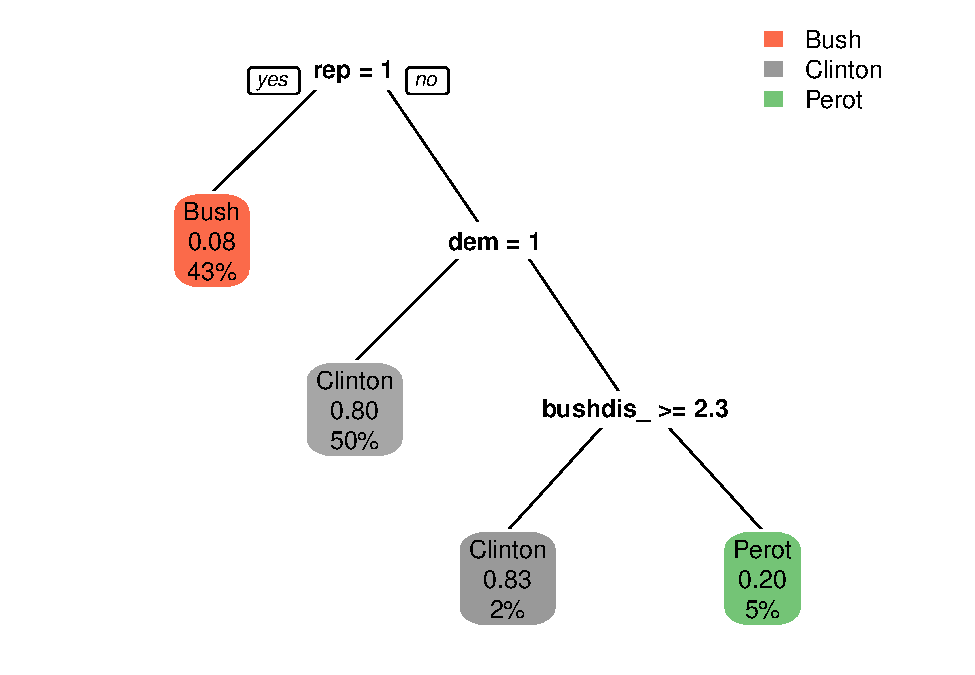
\includegraphics{1992-US-election_files/figure-latex/unnamed-chunk-14-2.pdf}
We decided to create a few models for the data set vote. We trained a
portion of the data set to create a lasso and ridge model. We also
created 3 logistic regression models. 2 that only have either
categorical or continues variables and the other one that has a
combination of both. We also trained a nother portion of the data set
for our decision tree and we created it.

\hypertarget{predictions}{%
\subsection{Predictions}\label{predictions}}

\begin{Shaded}
\begin{Highlighting}[]
\NormalTok{Accuracy }\OtherTok{\textless{}{-}} \ControlFlowTok{function}\NormalTok{(pred, real, }\AttributeTok{threshold =} \FloatTok{0.5}\NormalTok{)\{}
\NormalTok{  predClass }\OtherTok{\textless{}{-}}  \FunctionTok{ifelse}\NormalTok{(pred }\SpecialCharTok{\textgreater{}}\NormalTok{ threshold, }\DecValTok{1}\NormalTok{, }\DecValTok{0}\NormalTok{)}
\NormalTok{  acc }\OtherTok{\textless{}{-}} \FunctionTok{sum}\NormalTok{(predClass }\SpecialCharTok{==}\NormalTok{ real) }\SpecialCharTok{/} \FunctionTok{length}\NormalTok{(real)}
  \FunctionTok{return}\NormalTok{(acc)}
\NormalTok{\}}
\end{Highlighting}
\end{Shaded}

\begin{Shaded}
\begin{Highlighting}[]
\NormalTok{(acc1 }\OtherTok{\textless{}{-}} \FunctionTok{Accuracy}\NormalTok{(}\AttributeTok{pred =}\NormalTok{ pred.log1, }\AttributeTok{real =}\NormalTok{ vote}\SpecialCharTok{$}\NormalTok{vote\_num))}
\end{Highlighting}
\end{Shaded}

\begin{verbatim}
## [1] 0.3410341
\end{verbatim}

\begin{Shaded}
\begin{Highlighting}[]
\NormalTok{(acc2 }\OtherTok{\textless{}{-}} \FunctionTok{Accuracy}\NormalTok{(}\AttributeTok{pred =}\NormalTok{ pred.log2, }\AttributeTok{real =}\NormalTok{ vote}\SpecialCharTok{$}\NormalTok{vote\_num))}
\end{Highlighting}
\end{Shaded}

\begin{verbatim}
## [1] 0.3410341
\end{verbatim}

\begin{Shaded}
\begin{Highlighting}[]
\NormalTok{(acc3 }\OtherTok{\textless{}{-}} \FunctionTok{Accuracy}\NormalTok{(}\AttributeTok{pred =}\NormalTok{ pred.log3, }\AttributeTok{real =}\NormalTok{ vote}\SpecialCharTok{$}\NormalTok{vote\_num))}
\end{Highlighting}
\end{Shaded}

\begin{verbatim}
## [1] 0.3410341
\end{verbatim}

\begin{Shaded}
\begin{Highlighting}[]
\CommentTok{\# Brier Score}
\NormalTok{(BS.log1 }\OtherTok{\textless{}{-}} \FunctionTok{sqrt}\NormalTok{(}\FunctionTok{mean}\NormalTok{((vote}\SpecialCharTok{$}\NormalTok{vote\_num }\SpecialCharTok{{-}}\NormalTok{ pred.log1)}\SpecialCharTok{\^{}}\DecValTok{2}\NormalTok{)))}
\end{Highlighting}
\end{Shaded}

\begin{verbatim}
## [1] 0.6459124
\end{verbatim}

\begin{Shaded}
\begin{Highlighting}[]
\NormalTok{(BS.log2 }\OtherTok{\textless{}{-}} \FunctionTok{sqrt}\NormalTok{(}\FunctionTok{mean}\NormalTok{((vote}\SpecialCharTok{$}\NormalTok{vote\_num}\SpecialCharTok{{-}}\NormalTok{ pred.log2)}\SpecialCharTok{\^{}}\DecValTok{2}\NormalTok{)))}
\end{Highlighting}
\end{Shaded}

\begin{verbatim}
## [1] 0.6552625
\end{verbatim}

\begin{Shaded}
\begin{Highlighting}[]
\NormalTok{(BS.log3 }\OtherTok{\textless{}{-}} \FunctionTok{sqrt}\NormalTok{(}\FunctionTok{mean}\NormalTok{((vote}\SpecialCharTok{$}\NormalTok{vote\_num }\SpecialCharTok{{-}}\NormalTok{ pred.log3)}\SpecialCharTok{\^{}}\DecValTok{2}\NormalTok{)))}
\end{Highlighting}
\end{Shaded}

\begin{verbatim}
## [1] 0.6835589
\end{verbatim}

As we can see here the accuracy score for all the logistic regression is
the same. Since that is the case we need to focus on the brier score.
Which would mean that log1 which is the one that has both continouse and
catagorical variables in it is the best one of the bunch.

\begin{Shaded}
\begin{Highlighting}[]
\NormalTok{(accLasso }\OtherTok{\textless{}{-}} \FunctionTok{Accuracy}\NormalTok{(}\AttributeTok{pred =}\NormalTok{ y.predlog\_l1, }\AttributeTok{real =}\NormalTok{ y.test))}
\end{Highlighting}
\end{Shaded}

\begin{verbatim}
## [1] 0.3516484
\end{verbatim}

\begin{Shaded}
\begin{Highlighting}[]
\NormalTok{(accLRidge }\OtherTok{\textless{}{-}} \FunctionTok{Accuracy}\NormalTok{(}\AttributeTok{pred =}\NormalTok{ y.predlog\_r1, }\AttributeTok{real =}\NormalTok{ y.test))}
\end{Highlighting}
\end{Shaded}

\begin{verbatim}
## [1] 0.3516484
\end{verbatim}

\begin{Shaded}
\begin{Highlighting}[]
\NormalTok{(BS.logL1 }\OtherTok{\textless{}{-}} \FunctionTok{sqrt}\NormalTok{(}\FunctionTok{mean}\NormalTok{((y.test }\SpecialCharTok{{-}}\NormalTok{ y.predlog\_l1)}\SpecialCharTok{\^{}}\DecValTok{2}\NormalTok{)))}
\end{Highlighting}
\end{Shaded}

\begin{verbatim}
## [1] 0.6852876
\end{verbatim}

\begin{Shaded}
\begin{Highlighting}[]
\NormalTok{(BS.logL2 }\OtherTok{\textless{}{-}} \FunctionTok{sqrt}\NormalTok{(}\FunctionTok{mean}\NormalTok{((y.test }\SpecialCharTok{{-}}\NormalTok{ y.predlog\_r1)}\SpecialCharTok{\^{}}\DecValTok{2}\NormalTok{)))}
\end{Highlighting}
\end{Shaded}

\begin{verbatim}
## [1] 0.6852333
\end{verbatim}

With the Lasso and ridge model it is the same case the accuracy scores r
identical and since that is the case we need to choose the model with
the lowest brier score which would be the ridge model.

\begin{Shaded}
\begin{Highlighting}[]
\CommentTok{\# {-}{-}{-}{-}{-} Evaluating Prediction Quality {-}{-}{-}{-}{-}}
\CommentTok{\# Calculate performance with AUC and RMSE}
\FunctionTok{auc}\NormalTok{(vote.test}\SpecialCharTok{$}\NormalTok{vote\_num, pred.dt)}
\end{Highlighting}
\end{Shaded}

\begin{verbatim}
## Warning in roc.default(response, predictor, auc = TRUE, ...): 'response'
## has more than two levels. Consider setting 'levels' explicitly or using
## 'multiclass.roc' instead
\end{verbatim}

\begin{verbatim}
## Setting levels: control = 1, case = 2
\end{verbatim}

\begin{verbatim}
## Setting direction: controls < cases
\end{verbatim}

\begin{verbatim}
## Area under the curve: 0.9299
\end{verbatim}

\begin{Shaded}
\begin{Highlighting}[]
\NormalTok{( rmse }\OtherTok{\textless{}{-}} \FunctionTok{sqrt}\NormalTok{(}\FunctionTok{mean}\NormalTok{((vote.test}\SpecialCharTok{$}\NormalTok{vote\_num }\SpecialCharTok{{-}}\NormalTok{ pred.dt)}\SpecialCharTok{\^{}}\DecValTok{2}\NormalTok{)) )}
\end{Highlighting}
\end{Shaded}

\begin{verbatim}
## [1] 1.565776
\end{verbatim}

\begin{Shaded}
\begin{Highlighting}[]
\FunctionTok{Accuracy}\NormalTok{(}\AttributeTok{pred=}\NormalTok{pred.dt, }\AttributeTok{real=}\NormalTok{vote.test}\SpecialCharTok{$}\NormalTok{vote\_num)}
\end{Highlighting}
\end{Shaded}

\begin{verbatim}
## [1] 0.01845018
\end{verbatim}

\begin{Shaded}
\begin{Highlighting}[]
\CommentTok{\# Naive Classifier}
\NormalTok{baseline\_probability }\OtherTok{\textless{}{-}} \FunctionTok{sum}\NormalTok{(vote.train}\SpecialCharTok{$}\NormalTok{vote\_num }\SpecialCharTok{==} \DecValTok{1}\NormalTok{)}\SpecialCharTok{/}\FunctionTok{nrow}\NormalTok{(vote.train)}
\NormalTok{pred.baseline }\OtherTok{\textless{}{-}} \FunctionTok{rep}\NormalTok{(baseline\_probability, }\FunctionTok{nrow}\NormalTok{(vote.test))}

\FunctionTok{auc}\NormalTok{(vote.test}\SpecialCharTok{$}\NormalTok{vote\_num, pred.baseline)}
\end{Highlighting}
\end{Shaded}

\begin{verbatim}
## Warning in roc.default(response, predictor, auc = TRUE, ...): 'response'
## has more than two levels. Consider setting 'levels' explicitly or using
## 'multiclass.roc' instead
\end{verbatim}

\begin{verbatim}
## Setting levels: control = 1, case = 2
## Setting direction: controls < cases
\end{verbatim}

\begin{verbatim}
## Area under the curve: 0.5
\end{verbatim}

\begin{Shaded}
\begin{Highlighting}[]
\NormalTok{( rmse }\OtherTok{\textless{}{-}} \FunctionTok{sqrt}\NormalTok{(}\FunctionTok{mean}\NormalTok{((vote.test}\SpecialCharTok{$}\NormalTok{vote\_num }\SpecialCharTok{{-}}\NormalTok{ pred.baseline)}\SpecialCharTok{\^{}}\DecValTok{2}\NormalTok{)) )}
\end{Highlighting}
\end{Shaded}

\begin{verbatim}
## [1] 1.679247
\end{verbatim}

\begin{Shaded}
\begin{Highlighting}[]
\FunctionTok{Accuracy}\NormalTok{(}\AttributeTok{pred=}\NormalTok{pred.baseline, }\AttributeTok{real=}\NormalTok{vote.test}\SpecialCharTok{$}\NormalTok{vote\_num)}
\end{Highlighting}
\end{Shaded}

\begin{verbatim}
## [1] 0
\end{verbatim}

Here tbh i dont know wt to say lovis ;D

\end{document}
